\documentclass[english]{beamer}
\usepackage{makeidx}
\usepackage{color}
\usepackage{graphicx}
\usetheme{Goettingen}
\setbeamercovered{transparent}

\usenavigationsymbolstemplate{}
\AtBeginSection[]{
  \frame<beamer>{
    \frametitle{Next...}
    \tableofcontents[currentsection]
   }
}

\definecolor{ListingBorderColor}{gray}{0.55}
\definecolor{ListingBackgroundColor}{gray}{0.95}

\usepackage{babel}
\usepackage{hyperref}
\usepackage{enumerate}
\usepackage{enumerate}
\usepackage{longtable}
\usepackage[T1]{fontenc}
\usepackage{ucs}
\usepackage[latin1]{inputenc}
\usepackage{textcomp}
\usepackage{alltt}
\usepackage{listings}

\title{Git the basics}
\author{Bart Trojanowski, \href{mailto:bart@jukie.net}{bart@jukie.net}}
\institute{Jukie Networks Inc.}
\date{July 9th, 2008}

\setcounter{tocdepth}{1}


\newcommand{\mysection}[2]{
  \hypertarget{#2}{}
  \section{#1}
  \label{#2}
}
\newcommand{\mysubsection}[2]{
  \hypertarget{#2}{}
  \subsection{#1}
  \label{#2}
}


\begin{document}
% =====================================================================
\label{header}\hypertarget{header}{}
\frame{\maketitle}

% ---------------------------------------------------------------------
\begin{frame}
        \frametitle{Table of contents}
        \par\noindent
        \tableofcontents
\end{frame}

% =====================================================================
% =====================================================================
\mysection{Concepts}{_concepts}
% ---------------------------------------------------------------------
\begin{frame}
\frametitle{Concepts}
\begin{itemize}
        \item Source Control Management
                \begin{itemize}
                        \item track changes to files
                        \item repository / database of changes
                        \item working directory / current state
                \end{itemize}

        \pause{}
        \item Centralized SCM
                \begin{itemize}
                        \item server: single database
                        \item client: working directory \&{} state
                \end{itemize}

        \pause{}
        \item Decentralized SCM
                \begin{itemize}
                        \item anyone can be a server
                        \item repository coupled with working directory
                        \item complete history
                        \item disconnected operation
                \end{itemize}
\end{itemize}

\end{frame}

% =====================================================================
\mysubsection{SCM components}{_scm_components}

% ---------------------------------------------------------------------
\begin{frame}
\frametitle{SCM components}
\begin{columns}[t]
        \begin{column}{.5\textwidth}
                Working tree
                \begin{itemize}
                        \item directories
                        \item files
                \end{itemize}

        \end{column}
        \begin{column}[T]{.5\textwidth}
                \vspace{.2\textheight}
                \includegraphics[width=\linewidth]{repo-working-tree.eps}
        \end{column}
\end{columns}

\end{frame}

% ---------------------------------------------------------------------
\begin{frame}
\frametitle{SCM components}
\begin{columns}[t]
        \begin{column}{.5\textwidth}
                Repository contents
                \begin{itemize}
                        \item blobs
                \end{itemize}
        \end{column}
        \begin{column}[T]{.5\textwidth}
                \vspace{.2\textheight}
                \includegraphics[width=\linewidth]{repo-blob.eps}
        \end{column}
\end{columns}

\end{frame}

% ---------------------------------------------------------------------
\begin{frame}
\frametitle{SCM components}
\begin{columns}[t]
        \begin{column}{.5\textwidth}
                Repository contents
                \begin{itemize}
                        \item blobs
                        \item trees
                \end{itemize}
        \end{column}
        \begin{column}[T]{.5\textwidth}
                \vspace{.2\textheight}
                \includegraphics[width=\linewidth]{repo-tree.eps}
        \end{column}
\end{columns}

\end{frame}

% ---------------------------------------------------------------------
\begin{frame}
\frametitle{SCM components}
\begin{columns}[t]
        \begin{column}{.5\textwidth}
                Repository contents
                \begin{itemize}
                        \item blobs
                        \item trees
                        \item commits
                \end{itemize}
        \end{column}
        \begin{column}[T]{.5\textwidth}
                \vspace{.2\textheight}
                \includegraphics[width=\linewidth]{repo-commit.eps}
        \end{column}
\end{columns}

\end{frame}

% ---------------------------------------------------------------------
\begin{frame}
\frametitle{SCM components}
\begin{columns}[t]
        \begin{column}{.5\textwidth}
                Repository contents
                \begin{itemize}
                        \item blobs
                        \item trees
                        \item commits
                        \item ancestry
                \end{itemize}
        \end{column}
        \begin{column}[T]{.5\textwidth}
                \vspace{.2\textheight}
                \includegraphics[width=\linewidth]{repo-ancestry.eps}
        \end{column}
\end{columns}

\end{frame}

% ---------------------------------------------------------------------
\begin{frame}
\frametitle{SCM components}
\begin{columns}[t]
        \begin{column}{.5\textwidth}
                Repository contents
                \begin{itemize}
                        \item blobs
                        \item trees
                        \item commits
                        \item ancestry
                        \item tags
                \end{itemize}
        \end{column}
        \begin{column}[T]{.5\textwidth}
                \vspace{.2\textheight}
                \includegraphics[width=\linewidth]{repo-tags.eps}
        \end{column}
\end{columns}

\end{frame}

% ---------------------------------------------------------------------
\begin{frame}
\frametitle{SCM components}
\begin{columns}[t]
        \begin{column}{.5\textwidth}
                Repository contents
                \begin{itemize}
                        \item blobs
                        \item trees
                        \item commits
                        \item ancestry
                        \item tags
                        \item branches
                \end{itemize}
        \end{column}
        \begin{column}[T]{.5\textwidth}
                \vspace{.2\textheight}
                \includegraphics[width=\linewidth]{repo-branches.eps}
        \end{column}
\end{columns}

\end{frame}

% ---------------------------------------------------------------------
\begin{frame}
\frametitle{SCM components}
\begin{columns}[t]
        \begin{column}{.5\textwidth}
                HEAD
                \begin{itemize}
                        \item current checkout
                        \item points to branch
                        \item sometimes detached
                \end{itemize}
        \end{column}
        \begin{column}[T]{.5\textwidth}
                \vspace{.2\textheight}
                \includegraphics[width=\linewidth]{repo-head.eps}
        \end{column}
\end{columns}

\end{frame}

% ---------------------------------------------------------------------
\begin{frame}
\frametitle{SCM components}
\begin{columns}[t]
        \begin{column}{.5\textwidth}
                Index
                \begin{itemize}
                        \item ``staging area''
                        \item what is to be committed
                \end{itemize}
        \end{column}
        \begin{column}[T]{.5\textwidth}
                \vspace{.2\textheight}
                \includegraphics[width=\linewidth]{repo-index.eps}
        \end{column}
\end{columns}

\end{frame}

% =====================================================================
\mysubsection{SCM operations}{_scm_operations}

% ---------------------------------------------------------------------
\begin{frame}
\frametitle{SCM operations}
Bootstrap
\begin{itemize}
        \item init
        \item checkout
        \item switch branch
\end{itemize}

Modify
\begin{itemize}
        \item add, delete, rename
        \item commit
\end{itemize}

Information
\begin{itemize}
        \item status
        \item diff
        \item log
\end{itemize}

Reference
\begin{itemize}
        \item tag
        \item branch
\end{itemize}
\end{frame}

% ---------------------------------------------------------------------
\begin{frame}
\frametitle{Centralized SCM}
\includegraphics[width=\linewidth]{centralized.eps}
\begin{itemize}
        \item operations require \textcolor{red}{server}
                \begin{itemize}
                        \item single point of failure
                        \item bottleneck
                \end{itemize}
\end{itemize}
\end{frame}

% ---------------------------------------------------------------------
\begin{frame}
\frametitle{more SCM operations}
Decentralized
\begin{itemize}
        \item clone
        \item pull, fetch
        \item push
\end{itemize}
\end{frame}

% ---------------------------------------------------------------------
\begin{frame}
\frametitle{Decentralized SCM}
\includegraphics[width=\linewidth]{decentralized.eps}
\begin{itemize}
        \item anyone can be a server
\end{itemize}
\end{frame}

% =====================================================================
\mysubsection{Decentralization}{_decentralization}

% ---------------------------------------------------------------------
\begin{frame}
\frametitle{Decentralization}
\includegraphics[width=\linewidth]{cloning-1-upstream.eps}
\begin{itemize}
        \item public repository
\end{itemize}
\end{frame}

% ---------------------------------------------------------------------
\begin{frame}
\frametitle{Decentralization}
\includegraphics[width=\linewidth]{cloning-2-local.eps}
\begin{itemize}
        \item make a local clone
\end{itemize}
\end{frame}

% ---------------------------------------------------------------------
\begin{frame}
\frametitle{Decentralization}
\includegraphics[width=\linewidth]{cloning-3-topic.eps}
\begin{itemize}
        \item create topic ``branches''
\end{itemize}
\end{frame}

% ---------------------------------------------------------------------
\begin{frame}
\frametitle{Decentralization}
\includegraphics[width=\linewidth]{cloning-4-push.eps}
\begin{itemize}
        \item push changes between any repositories
\end{itemize}
\end{frame}

% ---------------------------------------------------------------------
\begin{frame}
\frametitle{Decentralization}
\includegraphics[width=\linewidth]{cloning-5-publish.eps}
\begin{itemize}
        \item publish changes to public server
\end{itemize}
\end{frame}

% ---------------------------------------------------------------------
\begin{frame}
\frametitle{Decentralization}
\includegraphics[width=\linewidth]{cloning-6-trusted.eps}
\begin{itemize}
        \item share changes with trusted peers
\end{itemize}
\end{frame}

% ---------------------------------------------------------------------
\begin{frame}
\frametitle{Is Decentralization any good?}

\begin{itemize}
        \item non-intrusive micro-commits
        \item detached operation
        \item no single point of failure
        \item backups are trivial
\end{itemize}
\end{frame}


% ---------------------------------------------------------------------
\begin{frame}
        END
\end{frame}

% =====================================================================
\end{document}
